% Template for PLoS
% Version 1.0 January 2009

\documentclass[10pt]{article}

% amsmath package, useful for mathematical formulas
\usepackage{amsmath}
% amssymb package, useful for mathematical symbols
\usepackage{amssymb}

% graphicx package, useful for including eps and pdf graphics
% include graphics with the command \includegraphics
\usepackage{graphicx}

% Need to have subfigures
\usepackage{subcaption}
\pdfpagebox5

% cite package, to clean up citations in the main text. Do not remove.
\usepackage{cite}

\usepackage{color}
\usepackage[squaren]{SIunits} 
%\usepackage{units}

% Use doublespacing - comment out for single spacing
%\usepackage{setspace} 
%\doublespacing


% Text layout
\topmargin 0.0cm
\oddsidemargin 0.5cm
\evensidemargin 0.5cm
\textwidth 16cm 
\textheight 21cm

% Bold the 'Figure #' in the caption and separate it with a period
% Captions will be left justified
\usepackage[labelfont=bf,labelsep=period,justification=raggedright]{caption}

% Use the PLoS provided bibtex style
\bibliographystyle{plos2009}

% Remove brackets from numbering in List of References
\makeatletter
\renewcommand{\@biblabel}[1]{\quad#1.}
\makeatother


% Leave date blank
\date{}

\pagestyle{myheadings}
%% ** EDIT HERE **

%% ** EDIT HERE **
%% PLEASE INCLUDE ALL MACROS BELOW
\usepackage[printonlyused]{acronym}
\usepackage{multicol}

%% END MACROS SECTION

\begin{document}

% Title must be 150 characters or less
\begin{flushleft}
{\Large
\textbf{Modeling Poplar Growth as a Short Rotation Woody Crop for Biofuels}
}
% Insert Author names, affiliations and corresponding author email.
\\
Quinn Hart$^{1,\ast}$,
Olga Prelipova$^{2}$,
Justin Merz$^{1}$,
Peter Tittmann$^{3}$, 
Bryan Jenkins$^{4}$
\\
$^{\textbf{1}}$ Department of Land, Air, and Water, University of Califonia, Davis, USA
$^{\textbf{2}}$ Department of Computer Science, University of Califonia, Davis, USA
$^{\textbf{3}}$ Department of Forestry, University of Califonia, Berkeley, USA
$^{\textbf{4}}$ Energy Institute, University of Califonia, Davis, USA
\\
%\\textbf{3} Author3 Dept/Program/Center, Institution Name, City, State, Country
$\ast$ E-mail: qjhart@ucdavis.edu
\end{flushleft}

% Please keep the abstract between 250 and 300 words
\section*{Abstract}

Being able to predict the growth and yield of these crop under various
environmental conditions is an important step in the development of
energy system that can incorporate these \ac{SRWC} as feedstocks.  In
this study, the \acf{3pg} model was modified for \ac{SRWC}, with the
inclusion of a coppicing model.  The model was then tested against a
number of previous studies found in the literature.  

% Please keep the Author Summary between 150 and 200 words
% Use first person. PLoS ONE authors please skip this step. 
% Author Summary not valid for PLoS ONE submissions.   
%\section*{Author Summary}

\section*{Introduction}

The goals of this research were to develop modifications to the
\ac{3pg} model to allow for an accurate representation of growth of
\ac{SRWC} over a range of environmental conditions, and to validate
the model compared to various field trials.

We are developing parameters to use the \acf{3pg} model as a means to
estimate poplar yields for the Pacific Northwest.  The model includes
basic processes for forest growth.  Modeling the physiological growth
is advantageous because it allows variation of poplar species
parameters and management practices.  Because it is a canopy carbon
balanced model, allocations for both above and below ground biomass
can be tracked for studies like life-cycle analysis.

The original \ac{3pg} model does not include coppicing as a management
practice, which is problematic as it cannot reasonably account for
post-coppicing regrowth.  The extended model includes coppicing with a
general model that allows a monthly growth contribution from an
existing root mass.  The model specifies a relatively small
contribution of aboveground growth from the accumulated root mass
after coppicing in order to initiate the next cycle of production.

The primary modification is the inclusion of a coppicing model for the
prediction of biomass production over the course of a number of
coppicing cycles.  The coppicing model introduced is a simple extension
that models the sprouting of the coppice, contribution to growth from
the existing root system, and modifications to the allocation of
resources based on the coppicing.

\begin{multicols}{3}[\section*{Acronyms}]
\addcontentsline{toc}{section}{Acronyms}
%\renewcommand{\baselinestretch}{1.0}
{\normalsize
\raggedright
%\setlength{\columnseprule}{1pt}
\begin{acronym}
\acro{gbsm}[\textsc{GBSM}]{Geospatial Bioenergy Systems Model}
\acro{3pg}[\textsc{3PG}]{Physiological Principles in Predicting Growth}
\acro{dW}[\ensuremath{\Delta W}]{Total Monthly Growth}
\acro{GIS}[\textsc{GIS}]{Geograhical Information System}
\acro{SRWC}[\textsc{SRWC}]{Short Rotation Woody Crops}
\acro{NPP}[\ensuremath{NPP}]{Net Primary Productivity}
\acro{LAI}[\ensuremath{LAI}]{Leaf Area Index}
\acro{RP}[\ensuremath{RP}]{Root Productivity}
\acro{NPPres}[\ensuremath{NPP_{res}}]{Residual desired $NPP$}
\acro{NPPt}[\ensuremath{NPP_{T}}]{$NPP$ if $LAI = LAI_{T}$}
\acro{dRres}[\ensuremath{\Delta R_{res}}]{Residual root contribution}
\acro{pRx}[\ensuremath{p_{R\%x}}]{Maximum root \%}
\acro{Rdp}[\ensuremath{R_{\Delta\%}}]{Root contribution}
\acro{W}[\ensuremath{W}]{Total plant mass}
\acro{WR}[\ensuremath{W_R}]{Total root mass}
\acro{fR}[\ensuremath{f_R}]{Root conversion efficiency}
\acro{fi}[\ensuremath{f_i}]{Generic growth limiters}
\end{acronym}
}
\end{multicols}

% You may title this section "Methods" or "Models". 
% "Models" is not a valid title for PLoS ONE authors. However, PLoS ONE
% authors may use "Analysis" 
\section*{Models}

\subsection*{Potential Growth Model}

Figure~\ref{fig:growth-model} shows and overview of the parts used in
the development of the poplar growth model. The model is based
primarily on the \ac{3pg} model~\cite{Landsberg1997,
  landsberg2010physiological}, with modifications for \ac{SRWC}.

\begin{figure}[!ht]
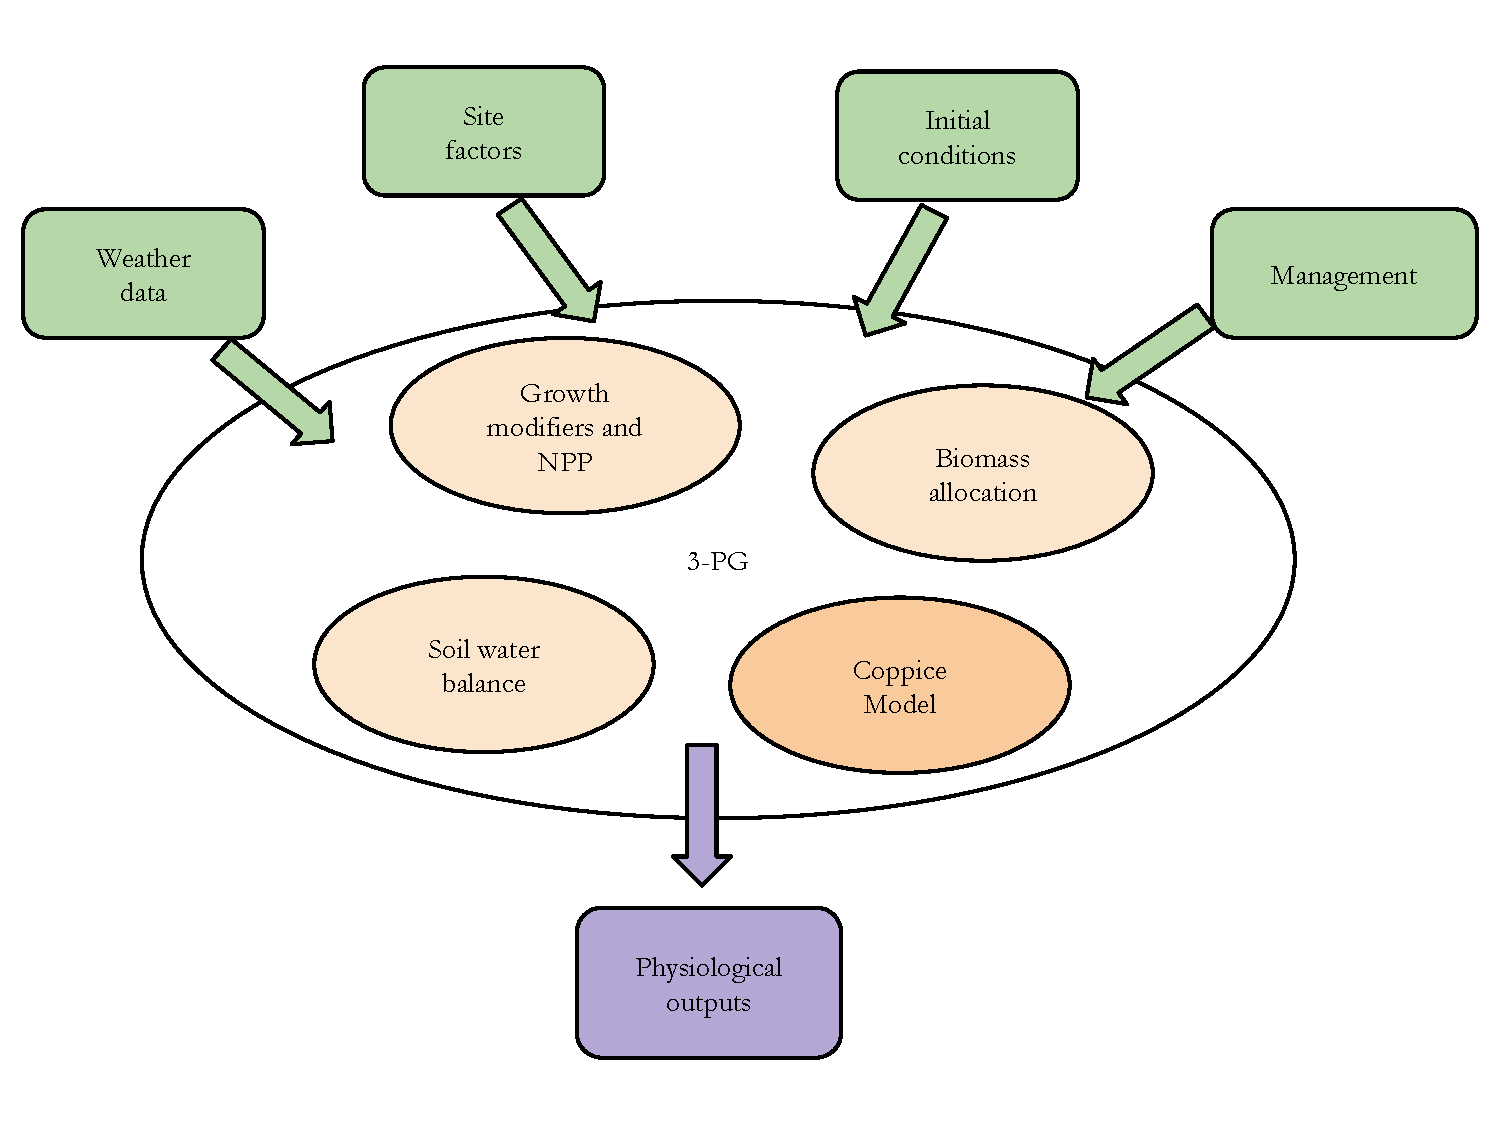
\includegraphics[width=1.0\linewidth]{model_overview}
\caption{ \textbf{\ac{3pg} Overview.}}
\label{fig:growth-model}
\end{figure}

The \acf{3pg} model takes as inputs weather data, site factors,
initial conditions, management practices, and species information.
The model runs at a monthly timestep. At each step the physiological
parameters are calculated and carried forward to the next month. Input
weather parameters are specified at the same monthly timestep, and
additional management parameters, such as irrigation scheduling, and
when the poplar is coppiced are also be included.

The physiological components of the \ac{3pg} model comprises of
submodules for estimating growth modifiers and \ac{NPP}, biomass
allocation, and soil water balance.  We have added an additional
module for regrowth after coppicing.

\subsubsection*{Poplar Hybrids}

A number of studies have been reported for modeling poplar using the
\ac{3pg} model.  The inputs used in this study draw from a number of
these studies.  The following table summarizes the base parameters
used for a generic poplar tree model.

\begin{table}[!ht]
\caption{\textbf{\ac{3pg} Model Tree Parameters}}
%\begin{tabular}{|c|c|c|}
\hline
Parameter & Source & value\\
\hline
\multicolumn{3}{|c|}{Greenwood Plantation Values}\\
type &  & ,\\
StockingDensity &  & 3587,\\
SeedlingMass &  & 0.0004,\\
pS &  & 0.1,\\
pF &  & 0,\\
pR &  & 0.9,\\
\hline
\multicolumn{3}{|c|}{Soil information based on current location}\\
maxaws &  & -1,\\
swpower &  & -1,\\
swconst &  & -1,\\
\hline
\multicolumn{3}{|c|}{ Weather Parameters}\\
month &  & -1,\\
tmin &  & -1,\\
tmax &  & -1,\\
tdmean &  & -1,\\
ppt &  & -1,\\
rad &  & -1,\\
nrel &  & -1,\\
daylight &  & -1,\\
\hline
\end{tabular}

\begin{tabularx}{\linewidth}{|c|X|c|}
  \hline
  Parameter & Source & Value\\
  \hline
  \acs{k}  & \acf{k} & 0.5\\
  fullCanAge [yr] & Year where tree reaches full Canopy Cover. & 0  \\
  kG \reciprocal\kilo\pascal & Determines the response of the canopy conductance to the vapor pressure deficit. & 0.5\\
  alpha [\kilogram\mole] & Canopy quantum efficiency. & 0.06\\
  \hline
  \acs{fT} [frac] & The parameters specifing limitations from ambient temperature. & \\
  $mn_{\acs{fT}}$ [\Celsius] & The minimum temperature for respiration & 5\\
  $opt_{\acs{fT}}$ [\Celsius] & The optimum temperature for respiration & 20\\
  $mx_{\acs{fT}}$  [\Celsius] & The maximum temperature for respiration & 40\\
  \hline
  \acs{BLcond} [\reciprocal\meter] & Canopy boundary layer conductance. Used in the calcuation of transpiration & 0.2\\
  \hline
  \acs{fAge} [frac] & Specifies the growth limiter as a function of the tree age.  This is a time dependant parameter. Specified with 4 parameters. & \\
  $f0_{\acs{fAge}}$ &  Value for \acs{fAge} at Initial Time & 1\\
  $f1_{\acs{fAge}}$ & Value for \acs{fAge} at Infinite Time & 0 \\
  $tm_{\acs{fAge}}$ [y] & Time in years where value is the average of $f0$ and $f1$ & 47.5\\
  $n_{\acs{fAge}}$ & $n>=1$ Parameter specifing the rate of change around tm.  n=1 is approximately a linear change, as n increases, change becomes more localized around tm. & 3.5\\
  \hline
   $fN0$ [frac] & Used in the calculation of the nutritional modifier,$fNutr$.  $fNutr$ ranges from [$fNO$,1) based on the fertility index which ranges from 0 to 1.  When $fN0=1$ indicates $fNutr=1$ & 1\\
   \hline
   \acs{SLA} [$\square\meter\per\kilogram$] & \acf{SLA}.  Defined as a function of the tree age.  Used in the calculation of LAI. &\\
   $f0_{\acs{SLA}}$ & \acs{SLA} at initial time & 10.8\\
   $f1_{\acs{SLA}}$ & \acs{SLA} at infinite timestep & 10.8\\
   $tm_{\acs{SLA}}$ [y] & Time in years where value is the average of $f0$ and $f1$ & 1\\
   $n$  & $n>=1$; Parameter specifing the rate of change around $tm$.  $n=1$ is approximately a linear change, as n increases, change becomes more localized around $tm$. & 2\\
   \hline
   $Cond$ [$\meter\per\second$] &  Canopy Conductance.  Along with a Physiological modifer, specifies the canopy conductance.  Used in calculation of transpiration & \\
   $mn_{Cond}$ & Minimum value, when $lai=0$ & 0.0001\\
   $mx_{Cond}$ & Maximum value & 0.02\\
   $lai_{Cond}$ [$\square\meter\per\square\meter$] & \ac{LAI} where parameter reaches a maximum value. & 3.33\\
 \hline
 $Intcptn$ [frac] & Rainfall interception fraction.  A linear function w.r.t. \ac{LAI} & \\
  $mn_{Intcptn}$ & Minimum value, when lai=0 & 0\\
  $mx_{Intcptn}$ & Maximum value & 0.15\\
  $lai_{Intcptn}$ [$\square\meter\per\square\meter$] & \ac{LAI} where parameter reaches a maximum value. & 5\\
 \hline \hline
 y & Assimilation use efficiency.  Used in calculation of the NPP. & 0.47\\
 \hline 
\end{tabularx}


\begin{flushleft}The table shows the data sources used for the
  modeling of the potential Growth model for poplar.
\end{flushleft}
\label{tab:3pg-tree}
 \end{table}


\begin{table}[!ht]
\caption{
\textbf{\ac{3pg} Model Plantation and Site Parameters}}
\begin{tabular}{|c|c|c|}
\hline
Parameter & Source & value\\
\hline
\multicolumn{3}{|c|}{Greenwood Plantation Values}\\
type &  & ,\\
StockingDensity &  & 3587,\\
SeedlingMass &  & 0.0004,\\
pS &  & 0.1,\\
pF &  & 0,\\
pR &  & 0.9,\\
\hline
\multicolumn{3}{|c|}{Soil information based on current location}\\
maxaws &  & -1,\\
swpower &  & -1,\\
swconst &  & -1,\\
\hline
\multicolumn{3}{|c|}{ Weather Parameters}\\
month &  & -1,\\
tmin &  & -1,\\
tmax &  & -1,\\
tdmean &  & -1,\\
ppt &  & -1,\\
rad &  & -1,\\
nrel &  & -1,\\
daylight &  & -1,\\
\hline
\end{tabular}

\begin{flushleft}The table shows the data sources used for the
  modeling of the potential Growth model for poplar.
\end{flushleft}
\label{tab:3pg-plantation-site}
 \end{table}


\subsection*{Coppicing Model}
\label{sec:coppicing-model}
The original \ac{3pg} model allocates mass produced from transpiration
into the the creation of new roots, stems and foliage.  In the
standard \ac{3pg} model, the amount allocated to stems is basically a
constant allocation, with a modifier due to the stress the plantation
is under.  In a \ac{SRWC} however, coppicing the trees during
harvesting introduces a situation where the stem and foliage are
removed, but the root ball remains.  The \ac{3pg} model has no
mechanism to increase to start re-growth from this stituation, or
moderate the allocations based on the coppiced plant.

\begin{figure}[!ht]
\begin{subfigure}[b]{.1125\linewidth}
\centering
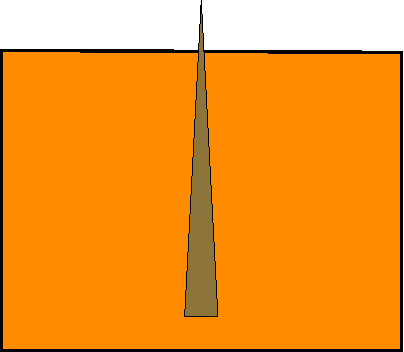
\includegraphics[width=1.0\linewidth]{img/tree_pics_1}
\caption{}  %\caption{planting}
\label{fig:grow_1}
\end{subfigure}
\begin{subfigure}[b]{.1125\linewidth}
\centering
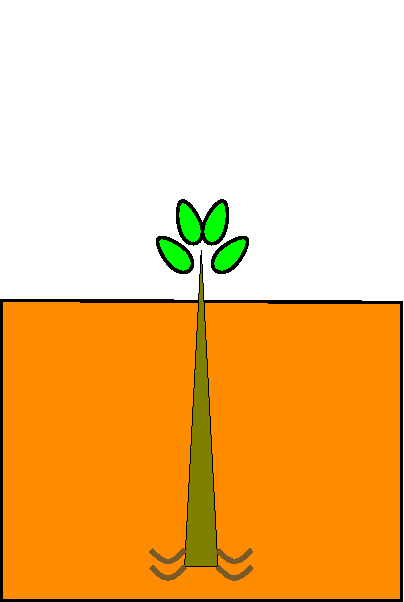
\includegraphics[width=1.0\linewidth]{img/tree_pics_2}
\caption{}  %\caption{sprout}
\label{fig:grow_2}
\end{subfigure}
\begin{subfigure}[b]{.1125\linewidth}
\centering
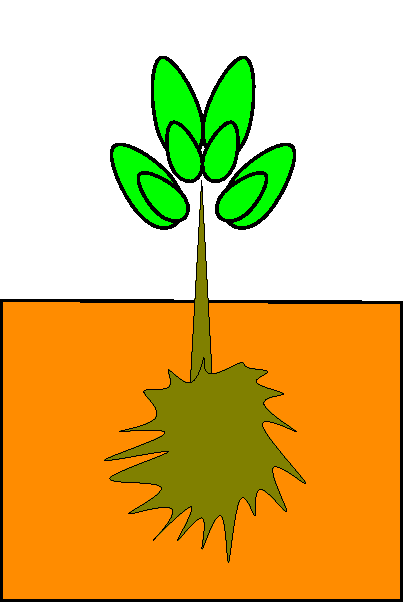
\includegraphics[width=1.0\linewidth]{img/tree_pics_3}
\caption{}  %\caption{growth}
\label{fig:grow_3}
\end{subfigure}
\begin{subfigure}[b]{.1125\linewidth}
\centering
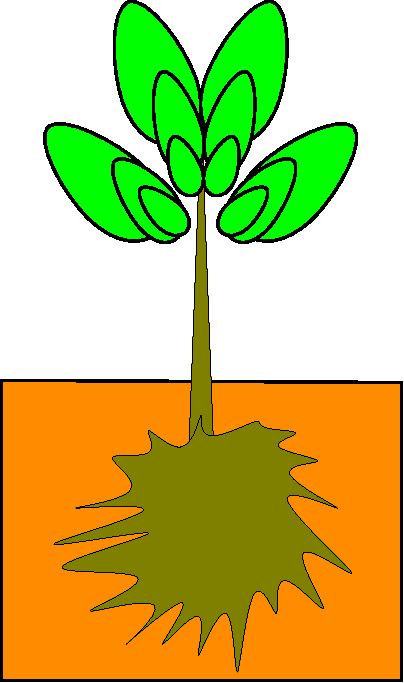
\includegraphics[width=1.0\linewidth]{img/tree_pics_4}
\caption{}  %\caption{maturity}
\label{fig:grow_4}
\end{subfigure}
\begin{subfigure}[b]{.1125\linewidth}
\centering
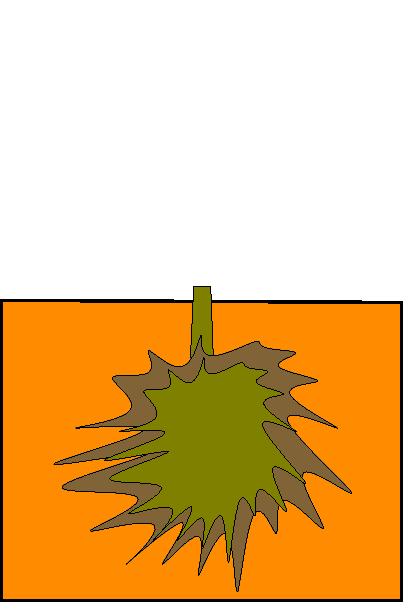
\includegraphics[width=1.0\linewidth]{img/tree_pics_5}
\caption{}  %\caption{coppiced}
\label{fig:grow_5}
\end{subfigure}
\begin{subfigure}[b]{.1125\linewidth}
\centering
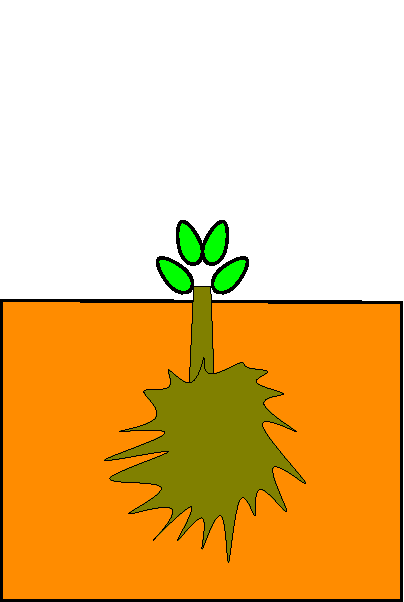
\includegraphics[width=1.0\linewidth]{img/tree_pics_6}
\caption{}  %\caption{resprouting}
\label{fig:grow_6}
\end{subfigure}
\begin{subfigure}[b]{.1125\linewidth}
\centering
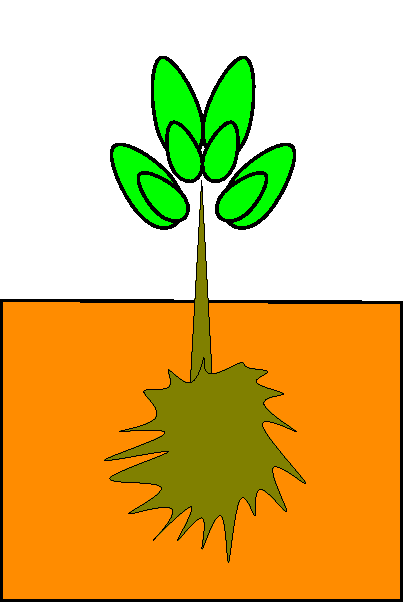
\includegraphics[width=1.0\linewidth]{img/tree_pics_7}
\caption{}  %\caption{regrowth}
\label{fig:grow_7}
\end{subfigure}
\begin{subfigure}[b]{.1125\linewidth}
\centering
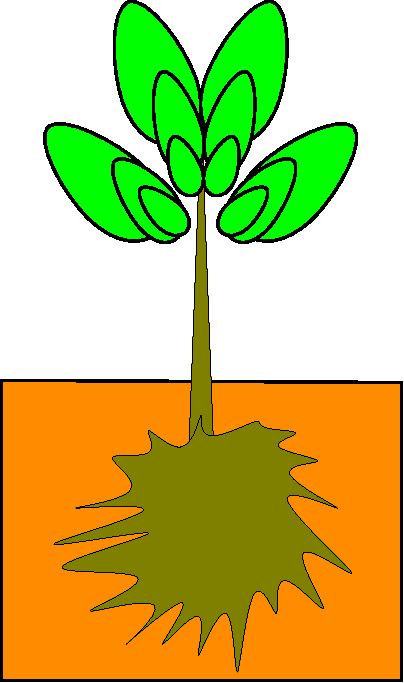
\includegraphics[width=1.0\linewidth]{img/tree_pics_4}
\caption{}  %\caption{next harvest}
\label{fig:grow_8}
\end{subfigure}
\caption{ \textbf{Poplar \ac{SRWC} growth.} The growth stages for poplar
  grown as an \ac{SRWC} with one coppicing cycle shown. }
\label{fig:grow}
\end{figure}

Figure~\ref{fig:grow} shows a figure of the growth of a poplar planted
as a \ac{SRWC}.  Poplars are propagated via cuttings of bare poplar
stem, mostly under the soil,~(Figure~\ref{fig:grow_1}).  The cutting
provides energy for the establishment of the seedling via buds above
and below the surface~(Figure~\ref{fig:grow_2}). As the poplar
matures, all growth comes from the productivity provided by the
foliage.  This includes the establishment of the root
ball~(Figure~\ref{fig:grow_3}).By the time the poplar is ready for
coppicing~(Figure~\ref{fig:grow_4}), the plants are well established.

After coppicing, there is a surfeit of root mass, and no foliage to
provide photosynthetic based productivity to the
tree~(Figure~\ref{fig:grow_5}).  Later, resprouting begins with the
root ball providing initial energy for the reestablishment of
seedlings~(Figure~\ref{fig:grow_6}) which then leads through the
maturation of the poplar, ready for the next
harvest~(Figures~\ref{fig:grow_7} and~\ref{fig:grow_8}).

We have developed a simple root interaction system to added to the
\ac{3pg} model to model the behavior both of the post-coppiced
situation as well as the initial planting of the cutting.  The model
basically allows for some additional production to come from the root
mass under certain conditions.

An Overview of the model is shown in figure~\ref{fig:coppice}.  Three
species specific parameters control the coppicing model.  These are
combined with some of the existing \ac{3pg} parameters to model the
extent and timing of regrowth from the coppiced plant.

\begin{figure}[!ht]
  \centering
\begin{subfigure}[b]{.2\linewidth}
  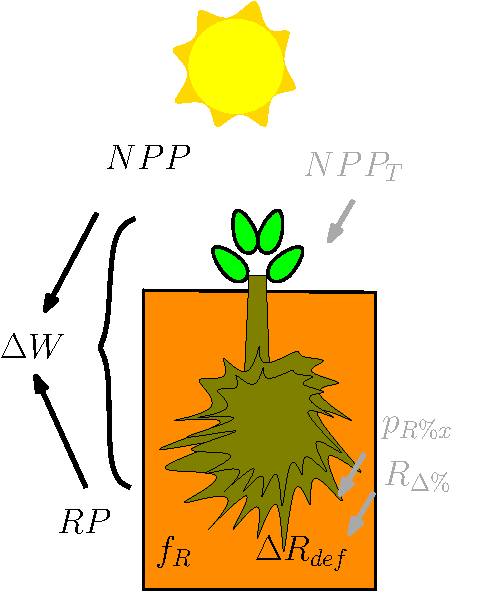
\includegraphics[width=1.0\linewidth]{img/tree_pics_10}
  \caption{Parameters}
  \label{fig:coppice-img}
\end{subfigure}
\quad
\begin{subtable}[b]{.75\linewidth}
\begin{align}
\acs{dW}=\acs{NPP}+\acs{RP} \\
\acs{RP} = \begin{cases} 0 & \acs{NPPres} <=0 \\
\acs{fR} ~ min (\acs{dRdef} ,\acs{NPPres}) & \acs{NPPres} > 0  
\end{cases} \\
\acs{NPPres} = \acs{NPPt}-\acs{NPP} \\
\acs{dRdef} = \acs{WR}(\acs{WR}/\acs{W} - \acs{pRx})\acs{Rdp}
\end{align}
\caption{Model Definition}
\end{subtable}
\caption{\textbf{Coppice Model Overview}}
  \label{fig:coppice}
\end{figure}

The \ac{3pg} model previously defined a maximum root size, \acs{pRx},
which is an upper limit on the root size with respect to the entire
plant size.  After coppicing, the actual root size is larger then,
\acs{pRx}.  The parameter, \acs{Rdp}, (ranging from 0 to 1), defines
what amount of this extra root can contribute to resprouting in a
given timestep.  A value of 0 indicates no root contribution for
regrowth, higher values indicate more potential growth available to
the plant at each timestep.

The growth contribution is also affected by the potential of a plant
to grow under the current weather conditions.  The seasonal timing of
the is moderated with the \acs{LAIt} parameter.  The \acs{LAIt}
parameter defines an operational \acs{LAI} which the plant attempting
to reach.  This affects the timing of the root contribution, because
for any given weather conditions, two versions of the plants \ac{NPP}
can be calculated, one at that plants current \acs{LAI}, and one at
the \acs{LAIt} level.  The difference in these values reflect the
targeted contribution of the root to regrowth.  As this value is
tied to the \ac{NPP}, regrowth is not made during times when the
foliage wouldn't contribute to more growth itself.  This method times
regrowth with climatic conditions that are favorable for growth.
\acs{LAIt} can vary from 0 and greater.  A value of 0 indicates no
root contribution, where higher values indicate contribution from the
roots even as the plant is producing higher values for \acs{NPP} from
it's foliage.

Finally, the parameter \acf{fR}, ranging from 0 to 1, determines the
efficiency of the contribution, in effect, determining the fraction of
new mass of growth, to loss of root mass.

In poplar plantations, the initial planting is modeled the same way,
with a different set of parameters to model the contribution from
planted poplar stick.

\subsubsection{Growth impacts}
\label{sec:growth-impacts}

As described in Section~\ref{sec:coppicing-model}, there are three
coppicing parameters that effect the regrowth of the trees after
coppicing.  \acs{Rdp} affects, \acs{pRx} and \acs{NPPres}.

\section*{Validation}

% Results and Discussion can be combined.
\section*{Results}

The \ac{3pg} model was tested with a number field tests found in the
literature.  Field tests that included one or more coppiced rotations
where included.  The model was used in the comparison of as many
parameters reported by the literature where possible.  

In each case, input weather conditions we obtained for the time of the
field work, and soil parameters were either obtained, or estimated
from the description in the literature.  

Genotype specific parameters were

Three field
\subsection{Pontailler 1999}
\label{sec:pont}

Pontailler~\cite{Pontailler1999}, described the results of biomass
measurements over 5 two year coppicing events for a five different
poplar species, grown in Orsay, France from 1987 through 1997.
Yields, post coppicing stems per stump, average height, and \ac{LAI}
were among the parameters measured.

Pontailler found consistent biomass returns on the plots for the most
part, and attributed differences, especially the lower returns in
1991-1992, as due to drought conditions for the region.  The \ac{3pg}
model was assigned parametric variations due to genotype.  These are
shown in table~\ref{tab:pont-3pg}.

\begin{table}[!ht]
  \centering
%  \begin{tabular}{}    
%  \end{tabular}
  \caption{\ac{3pg} parameter variations of \ac{3pg} among genotypes}
  \label{tab:pont-3pg}
\end{table}

\begin{figure}[!ht]
  \centering

  \caption{Comparison of model to measurements for yearly growth over five
    coppicing events.}
\label{fig:pont-biomass}
\end{figure}


\subsection*{Proe 2002}

Proe~\cite{Proe2002} described  the results  of a number  of different
\ac{SRWC}  field  trials, including  annual  measurements of  biomass,
root:shoot  ratio, leaf/stem  ratios, LAI,  PAR and  other parameters.
Light interception was measured  seasonally as well.  The studies were
developed over a  5 year period in central  Scotland from 1989 through
1999. Coppiced and single stem  comparisons were made, but only for the
affects of  early coppicing  after one year.   Proe found  increase in
biomass production  for more closely spaced  plantings still noticeable
up to the 5th year of the study.

Comparisons the the \ac{3pg} model where made by replicating the three
plantings under the conditions described.  Weather information for the
Scotland field plots were determined from ?.  Comparisons were made
between the \ac{3pg} model and the measured values, for spacings of 1m and
1.5m, and the single stem, and the coppicing methods.  Comparisons of
the total biomass, LAI, and light interception were made.

\begin{figure}
  \centering
  
  \caption{Woody and Stem biomass predictions vs. Measurements}
  \label{fig:proe-wood}
\end{figure}

\begin{figure}[!ht]
  \centering
  
  \caption{LAI and Light interception predictions vs. measurements}
  \label{fig:proe-light}
\end{figure}

\cite{proe02} compare the results of two stocking densities

To compare comparison with the
model, it's 

There have been a few studies



\subsection{Afas 2008}
\label{Afas2008}

Starting in 1996, Afas,~\cite{Afas2008a} studied 17 types of poplar
over the course of 11 years for a field study in Belgium.  The study
included measurements of three separate coppicing events.  The study
found relatively high mortality rates for some of the genotypes.
Comparisons between the \ac{3pg} and measured values were made for the
genotypes with a survival rate of over 85\%.  No measurements of below
ground biomass were included.  Afas did propose an alimetric
relationship for non-destructive biomass estimations based on diameter
measurements of the stems from the stool.

Variations among the genotypes were estimated with changes to the \ac{3pg}
input parameters of : ?

\begin{table}[!ht]
  \centering
%  \begin{tabular}{}
    
%  \end{tabular}
  \caption{\ac{3pg} parameter variations of \ac{3pg} among genotypes}
  \label{tab:afas-3pg}
\end{table}

\begin{figure}[!ht]
  \centering

  \caption{Comparison of model to measurements for yearly growth over three
    coppicing events.}
\label{fig:afas-biomass}
\end{figure}

\section*{Management Considerations}
\label{sec:management-reg}

In wood energy plantations, the management regime impacts the time
between harvest, the fraction of the total biomass that enters the
supply chain, and growth rates. Coppice style management generally
suggests the use of a continuous harvest machine (forage harvester) at
3-5 year intervals over a 12-18 year rotation. Following coppice
harvest the stumps are left to re-sprout and will be harvested again
after 3-5 years.  Stem biomass that enters the feedstock supply chain
under coppice management is determined by the year of first entry
which determines stump volume.  Stump volume under coppice management
is not considered to enter the supply chain at any point in the
rotation. Round wood production implies the use of a piece-wise
(harvester) or semi piece-wise harvesting equipment
(feller-buncher). If stem diameter at harvest exceeds $\approx$ 8-10
cm, piece-wise harvesting is necessary. Following roundwood harvest,
the field will be cleared and preparedn for re-planting.

% Experimental work has suggested that there may be advantages to
% intercropping coppice and roundwood production. \emph{WHY?}. Under
% intercropping regime supply chain loss is determined by the combined
% loss from coppiced stumps and roundwood stumps over the rotation
% period.

\subsubsection*{Stocking Density}
\label{sec:stocking-density}

Initial stocking density is an important consideration, as planting
density is a primary driver in initialization costs, and need to be
recouped with gains in biomass production.  \ac{SRWC} differ from
more traditional plantations in the the total biomass is important
rather than the biomass per stem.  Actually, the fact that coppicing
results in more stems per stump can lead to efficiencies in the
harvesting 

\subsubsection*{Stump volume}
\label{sec:stump-volume}

The \ac{3pg} growth model estimates partitioning of biomass between stem,
leaf, and roots within a spatial domain defined by model input
parameters. Harvesting results in the collection of a fraction of the
total accumulated stem biomass into the feedstock supply chain for
energy production. The fraction of the biomass retained depends upon
the management regime. Stump, and saw kerf acount for the fraction of
stem biomass that is not captured in the supply chain.

Stump volume was determined using total tree volume predicted by \ac{3pg},
a stem taper function from for young poplar stands
\cite{Benbrahim2003} , and allometric relationships between total
biomass and diameter at breast height ($dbh$) \cite{Brahim2000}. The
taper equation was used to establish stem diameter at stump height,
and basal diameter, both of which which are necessary for determining
stump volume. Allometric biomass relationships in forestry are
generally described as in ~(\ref{form}).
\begin{equation}
  \label{eq:form}
  X=aY^b
\end{equation}

First, $dbh$ is calculated from tree mass $M$
\begin{equation}
    \label{eqn:dbh}
    dbh=aM^b
    \end{equation}

as in (\ref{eqn:form}) where $a=0.122$ and $b=2.38$ from \cite{Landsberg1997}.

We the calculate total tree height ($H$) using coefficients provided by \cite{Brahim2000}
\begin{equation}
    \label{eqn:height}
    \begin{bmatrix}\frac{14705.8823529412 M + 250.0 d^{2.34} -56617.6470588235}{D^{2.34}}\end{bmatrix}
    \end{equation}where $D$ is $dbh$ for the individual tree and $d$ is the stand average $dbh$. The use of stand average can improve the accuracy of the relationship, however as the 3-PG model does not predict variation in $dbh$ between stands we simply use the derived $dbh$ from \ref{eqn:dbh} fro both values. \cite{Benbrahim2003} also provides (\ref{eqn:taper}) to determine diameter at a given height or height at a given diameter:
\begin{equation}
    \label{eqn:taper}
    0=-d+\left(b_d-b_d\left(\frac{\log{\frac{1-h}{Ha}}}{-b}\right)^{1/c}\right)
    \end{equation}The taper equation provided by \cite{Benbrahim2003} also requires a basal diameter ($b_d$). We calculate $b_d$ modifying equation (\ref{eqn:taper}) using coefficients provided and $H$, $dbh$ from above. Using a stump height of 10.0 cm we calculate the top stump diameter with which we can calculate the stump volume.
\begin{equation}
    \label{eqn:sectionvolume}
    V=\left(\frac{l\pi}{12}\right)(d_1^2+d_a^2+d_1d_2)
    \end{equation}We then calculate stump mass using a wood density of 0.38 $g \cdot cc^{-1}$ and compare with total tree mass $M$
\subsubsection*{Stump volume regression}
To determine a simplified relationship between tree volume and stump volume we derive coefficients $a$ and $b$ in (\ref{eqn:form}) using a the ratio of stump mass to total stem mass over a range of stem volumes based on the allometric relationships in section \ref{sec:allo}.\begin{figure}[h]
     \centering
%    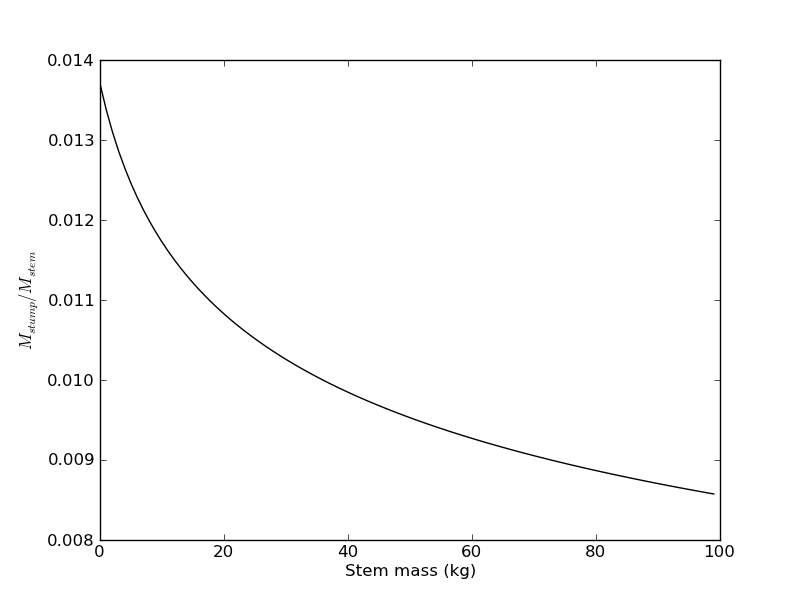
\includegraphics[width=0.5\textwidth]{nlm_stump.png}
    \caption{Stump to stem volume ratio as a function of stem volume}
    \label{fig:stump_vol}
    \end{figure}
Coefficients used in calculating stump volume as a function of total stem volume were found to be $a=0.0179877356445$ and $b=-0.169054308617$.

%\section*{Discussion}

\subsubsection{Predictions}

The \ac{ahb} project uses the above model to develop an estimate of
the potential yield of poplar throughout the study area.  Potential
yield maps only take into consideration the climatic, environmental
and phenological aspects.  They do not include the technical
considerations of the technical feasibility of poplar as a crop.
However, because management regimes effect poplar growth rates over
the period of the rotation different harvesting patterns are included
in the potential growth models.  The two practices considered were 12
year cycled harvesting, and 4 four year coppicing cycles.

The potential growth model implemented the \ac{3pg} forest growth
model over the study area, by implementing the \ac{3pg} model within a
\ac{GIS}.  \ac{3pg} modeled the growth of the poplar over a 12 year
cycle, ether with or without the coppicing cycles.  

Table~\ref{tab:3pg-grids} shows the required input grid parameters for
the \ac{3pg} model.  In addition, the model requires a number of other
parameterizations, primarily for the modeling of the forest. Table

\begin{table}[!ht]
\caption{
\textbf{Modeling Grids}}
\begin{tabular}{|c|c|c|}
\hline
Parameter & Units & Source \\
\hline
elevation & \meter & \\
\hline
precipitation & \milli\meter & \\
\hline
temperature & \celsius & \cite{prism-temp} \\
\hline
humidity & \unit{\%}  & \\
\hline
radiation & \mega\joule\per\squaremetre\usk\dday &  \\
\hline
sub-freezing days & \dday  & \\
\hline
\end{tabular}
\begin{flushleft}The table shows the data sources used for the
  modeling of the potential Growth model for poplar.
\end{flushleft}
\label{tab:3pg-grids}
 \end{table}




% Do NOT remove this, even if you are not including acknowledgments
\section*{Acknowledgments}
This project was funded by the USDA's Advanced Hardwood Biofuels for
the Pacific Northwest project, Number \#.

%\section*{References}
% The bibtex filename
\bibliography{ahb-pnw}

\section*{Figure Legends}

Move Figures here at the end.

\section*{Tables}

Move Table here at the end.

%% \begin{table}[!ht]
%% \caption{
%% \textbf{Title}}
%% \begin{tabular}{|c|c|c|}
%% table information
%% \end{tabular}
%% \begin{flushleft}Caption
%% \end{flushleft}
%% \label{tab:}
%%  \end{table}

\end{document}
